\section{A Validation-First Measurement Protocol (C1)}

No quantity enters this paper until it has passed three gates, in order, and the
gates are stated in general terms rather than tailored to the one domain we
demonstrate them on (Fig.~\ref{fig1}).

\textbf{G1: metric validity.} A resilience metric must (a) recover a
ground-truth planted value in synthetic data, (b) distinguish real measurements
from randomised controls, and (c) respond to the construct it claims to measure.
Six candidate resilience metrics were screened against three pre-registered
criteria --- rank recovery against a planted truth \emph{without} collapsing onto
another metric's truth, calibration whose slope interval covers 1 and intercept
interval covers 0, and separation from a week-permuted null. \textbf{Each
criterion passes two of the six metrics, and no metric passes all three.} The
metric with the highest own-truth correlation (\texttt{recovery\_time}, Spearman
0.9859) fails the rank criterion precisely because it is indistinguishable from
\texttt{centrality\_redistribution} (max $|$cross-Spearman$|$ = 0.8407 $\geq$
0.8). The two metrics that pass the rank criterion fail the permutation
criterion by construction, since a time-invariant structural quantity cannot
separate from a week-permuted control.

\textbf{Reporting a failure is itself a result.} Because the artifact lists the
three criteria without stating a conjunction rule, any single count of survivors
is a post-hoc choice, so we report the per-criterion matrix rather than a score
(Supplementary Note S2). A metric that fails is either not reported or reported
together with its failure; the six metric \emph{names} come from the
pre-registered plan while their operational definitions are ours, so none of
this validates the delivered measure.

\textbf{G2: instrument validity.} An estimator or predictor must be paired with
controls that \emph{can} reject it: a negative-control band with a pre-registered
usable window \citep{lipsitch2010negative}, permutation tests, and a
shuffled-label control repaired against feature-side separability. Every design
is registered before it is run \citep{nosek2018preregistration}. A control whose
value is fixed by construction is not a control, because G2 requires
demonstrating that the control varies within the stratification the metric uses.
We found that failure three times: in two single-feature arms whose retained
feature is constant within every bin, and in a de-leakage configuration whose
retained feature set is the stratifying variable itself. A control in that state
fails G2 by definition rather than by a margin, and a design that reports it as a
pass has not tested anything.

\textbf{G3: auditability.} Every reported number maps to a hash-verified
artifact in a manifest, or is flagged as not yet in it, and cross-artifact
quantities must be reproduced independently by two pipelines before they are
used. The manifest's domain is the result artifacts this study produced and its
time point is its own build; the boundary rule is reproduced with the manifest so
that the count can be recomputed rather than taken on trust (Supplementary Note
S1). Two pipelines independently reproduced an address count of
\textbf{61,487}, the rare cross-artifact agreement that licenses a reading.

CPU and GPU replicates are never tabulated together: on one replicate the
largest per-cell absolute difference in reported AUC was max $|d|$ = 0.0068
against a pre-registered tolerance of 1e-3. Device-equivalence checks under fp64
deterministic mode reproduce bitwise across devices, whereas fp32 forward passes
exhibit chaos amplification and are excluded from equivalence gates. Discipline
of this kind is what makes a negative result interpretable, and what allows a
failed instrument to be reported as a diagnosis rather than as a gap.

\textbf{The two-list rule.} When an instrument self-reports failure, the failure
report itself is that gate's output and must be given: how many cells fell
outside the window, which cells they were, what the window was, and the verbatim
decision rule. What is forbidden is any quantity \emph{read off} the failed
instrument --- a point estimate, a band, a comparison, a significance statement.
The test for which list a reading belongs to is whether it can stand without the
failed instrument: cell identities and the window cannot and are therefore
reportable, whereas a shuffled-control AUC can and is therefore withheld.

\textbf{The feature-side separability trap.} G2 is where existing practice is
thinnest, because a control that cannot reject anything looks exactly like a
control that rejected nothing. In censored ecological graphs, labels are
frequently derived from the same structural statistics that are also features ---
degree, transaction counts, address statistics --- so shuffling the labels does
not break the feature--label association and a shuffled-label control reads far
above chance. The instrument that did not fail here is the permutation null: it
uses \textbf{4000 draws}, one band per pre-registered horizon, and permutes time
steps rather than nodes. On our data the shuffled-label control reads
\textbf{0.71364} at $\Delta = 1$ against a permutation band of
\textbf{[0.4852, 0.5148]}, and the instrument's verdict is OUTSIDE.

\textbf{What anchors 0.5.} A control whose score is independent of the label
\emph{by construction}, read through the same within-entry-step weighted
estimator the arms are judged on, reads 0.4897--0.5141 (largest absolute
deviation 0.01406). So on this data \textbf{0.5} is the right anchor and the
shuffled control's distance from it is real. What that distance does \emph{not}
license is calling it leakage, because the excess conflates feature-side
separability with label leakage, is not decomposable, and is therefore not
published as any number.

\textbf{How far the repair goes.} Readings are within-entry-step weighted at
$\Delta = 1$. Dropping the calendar column reads 0.71556 and dropping the
position column reads 0.71758 --- both \emph{higher} than the as-built
\textbf{0.71364}, so removing either column repairs nothing. The attribution is
carried by the two arms that move the reading by more: the six family-mean
features alone read 0.69372 and the two family-count features alone read 0.56115.

Retraining on reduced feature families does not return the control to chance:
the strongest non-vacuous configuration moves the reading from \textbf{0.71364}
to \textbf{0.6561} and stops there (configuration-by-configuration accounting in
Supplementary Note S3). Two arms read exactly 0.5, but that is a construction
artefact: a single feature constant within every bin yields an AUC of exactly
one half, so those are vacuous controls rather than evidence of cleanliness. The
transferable lesson is that in this measurement domain a shuffled-label control
is not automatically a null model, and the first thing to check is whether it can
vary at all.

\begin{figure}[htbp]
\centering
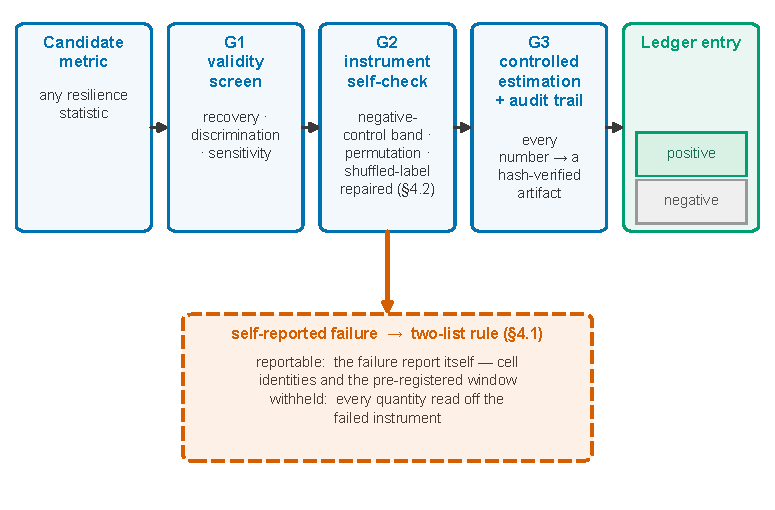
\includegraphics[width=0.78\textwidth]{figures/02_protocol_flow.pdf}
\caption{The five-step protocol. A candidate metric enters the G1 validity
screen and, if it survives, the G2 instrument self-check, then controlled
estimation with its audit trail (G3), ending in a ledger entry that records a
positive or a negative result. The red side branch is the protocol's most
distinctive move: when an instrument self-reports failure at G2, the failure
report itself becomes that gate's output under the two-list rule, while every
quantity read off the failed instrument is withheld.\label{fig1}}
\end{figure}
